\documentclass[11pt]{article}
\usepackage[margin=1in]{geometry}
\usepackage[T1]{fontenc}
\usepackage{lmodern,microtype}
\usepackage{amsmath,amssymb,graphicx,booktabs,array}
\usepackage{caption,hyperref}
\hypersetup{colorlinks=true,linkcolor=black,citecolor=black,urlcolor=blue}
\captionsetup{font=small,labelfont=bf}
\makeatletter
\setlength{\@fptop}{0pt}
\setlength{\@fpsep}{18pt}
\makeatother
\setlength{\parskip}{4pt}
\setlength{\parindent}{0pt}
\setlength{\emergencystretch}{3em}
\renewcommand{\floatpagefraction}{0.8}
\renewcommand{\topfraction}{0.9}
\renewcommand{\textfraction}{0.08}
\newcommand{\vorpFiveFamily}{Regularized linear}
\newcommand{\vorpFivermse}{3.664}
\newcommand{\vorpFivemae}{2.174}
\newcommand{\vorpFiverTwo}{-0.007}
\newcommand{\minutesFiveFamily}{Three-family ensemble}
\newcommand{\minutesFivermse}{3,443.517}
\newcommand{\minutesFivemae}{2,904.157}
\newcommand{\minutesFiverTwo}{0.046}
\newcommand{\activeFiveFamily}{Three-family ensemble}
\newcommand{\activeFivermse}{1.459}
\newcommand{\activeFivemae}{1.245}
\newcommand{\activeFiverTwo}{0.015}
\newcommand{\rotationFiveFamily}{Three-family ensemble}
\newcommand{\rotationFivebrier}{0.227}
\newcommand{\rotationFiveauc}{0.631}
\newcommand{\rotationFiveap}{0.566}
\newcommand{\starterFiveFamily}{Extra Trees}
\newcommand{\starterFivebrier}{0.176}
\newcommand{\starterFiveauc}{0.646}
\newcommand{\starterFiveap}{0.344}
\newcommand{\SampleN}{663}
\newcommand{\TestN}{98}
\newcommand{\DevelopmentN}{372}
\newcommand{\CollegeN}{65,649}
\newcommand{\FocalTarget}{Five-year minutes}
\newcommand{\CheckN}{35}
\newcommand{\ValidCheckN}{34}
\newcommand{\TrialN}{1095}
\title{Forecasting Five-Year NBA Value and Participation\\Among NCAA Draftees:\\Chronological Validation of College and Combine Predictors}
\hypersetup{pdftitle={Forecasting Five-Year NBA Value and Participation Among NCAA Draftees: Chronological Validation of College and Combine Predictors},pdfauthor={Kota Shida}}
\author{Kota Shida}
\date{October 13, 2026}

\begin{document}
\maketitle
\begin{abstract}
Can public college statistics and draft-year measurements forecast five-year NBA value and participation? We reconstruct \SampleN{} school-confirmed NCAA draftees from 2008--2021 using \CollegeN{} college player-season records and historical draft archives, without an NBA-performance inclusion threshold. The outcomes are cumulative Value Over Replacement Player (VORP), minutes, years active, sustained rotation service, and sustained starter service. Regularized linear models, forests, boosted trees, and equal-weight ensembles use chronological validation with a five-year label-maturity gap. Feature sets compare college production, engineered histories, and combine measurements; preprocessing and target transformations are fitted within training folds. On the frozen \TestN{}-player 2020--2021 test, the selected VORP model has RMSE \vorpFivermse{} versus 3.655 for the training mean, with $R^2=\vorpFiverTwo{}$. Minutes, years active, and rotation show modest reductions in point-estimate error; starter Brier score worsens. Rotation Brier score is \rotationFivebrier{} versus 0.240 for the prevalence baseline, with AUC \rotationFiveauc{}. All five paired bootstrap intervals include zero. Actual draft order, evaluated separately as post-selection information, forecasts service outcomes more accurately. The contribution is an auditable retrospective benchmark with an explicit information clock. The evidence does not establish dependable predictive gains or a substitute for scouting, and its scope is limited by two test cohorts and incomplete independent source verification.
\end{abstract}

\section{Introduction}
An NBA prospect's professional future depends on both basketball ability and the opportunity to use it. A player can survive several seasons without accumulating substantial value, produce efficient minutes in a limited role, or become a high-volume starter. These outcomes are related but not equivalent. A prospect model should therefore identify its decision target rather than label all professional achievement ``success.''

College basketball offers unusually detailed amateur production records, including exposure, shooting attempts, playmaking, rebounding, defensive events, and box-score estimates of impact. Physical combine measurements provide a complementary description of a prospect's tools. The challenge is to determine whether these public predictors generalize to future draft classes, not merely whether they explain a pooled historical sample.

This study asks three questions. First, how much can dated college production predict five-year NBA value and service, conditional on a player eventually being drafted? Second, do engineered college trajectories and physical measurements improve chronological predictive performance? Third, which definitions of five-year success are empirically learnable with these sources? We compare targets within a common protocol while retaining all outcomes in the final report. We do not change the research question to whichever final-test score looks strongest.

The contribution is an auditable retrospective benchmark, rather than a new prediction algorithm. It checks college identity against independently listed draft schools, separates actual draft position from pre-selection predictors, and evaluates five outcomes under a common label-maturity rule. Earlier studies already examine college-to-NBA translation and service outcomes. Here the emphasis is on what those predictors deliver when five-season follow-up must be complete at each simulated forecast date. This constraint does not establish that every archived metric definition or source release existed at that historical date.

\section{Literature Review}
Research on draft forecasting motivates a college-centered model without establishing that any algorithm must be superior. Coates and Oguntimein study college production, professional outcomes, and career length among historical draftees, highlighting the distinction between productivity and durability \cite{coates}. Their completed-career design addresses a different estimand from a fixed-window prospective forecast.

Moxley and Towne analyze early NBA trajectories and forecast later draft classes using a growth-mixture framework. Their results associate stronger trajectories with college performance, program quality, and youth, rather than demonstrating a general advantage for athletic ``potential'' measures \cite{moxley}. Kannan et al. combine college statistics, biometrics, position, and draft selection order for NBA success prediction \cite{kannan}. Draft position is informative, but including it changes the prediction date and blends amateur information with professional selection decisions.

Teramoto et al. use principal components and robust regression to investigate combine measurements and first-year and three-year professional performance \cite{teramoto}. Li and Cao find weak relationships in a small recent rookie sample \cite{li}. These studies motivate a physical-feature ablation rather than a presumption that height, speed, or jumping ability will reliably improve five-year forecasts. Wieth\"uchter's college-based survival study distinguishes rookie-contract survival, rotation and starter service, and impact thresholds \cite{wiethuchter}. The distinction supports evaluating multiple operational targets; player-level aggregation alone does not establish chronological label availability.

Czasonis et al. use relevance-weighted outcomes of earlier draftees to forecast rookie-year VORP and minutes from physical attributes, final college production, and college and NBA team context \cite{czasonis}. Their illustration includes college draftees who appeared in the NBA and concerns a one-season horizon. It establishes related chronological forecasting work, while our study uses a fixed five-season window and retains assumed nonparticipants. Differences in populations, predictors, horizons, and evaluation procedures prevent direct comparisons of reported accuracy.

More recently, Milo\v{s}evi\'{c} et al. predict career-status categories using the first one, three, or five NBA seasons \cite{milosevic}. Their predictors become available after professional entry, so their classification results answer a later forecasting question. Together, these studies make multiple outcomes and flexible models established choices. Our narrower addition is a school-confirmed, draft-anchored reconstruction with maturity-constrained selection and explicit negative baseline comparisons; we do not claim the first use of college statistics, combine data, or machine learning for NBA prediction.

Flexible methods can capture nonlinear translation from college roles to professional opportunity. Random Forests average randomized trees \cite{breiman}; XGBoost and LightGBM implement regularized boosted trees \cite{xgboost,lightgbm}; CatBoost provides an alternative boosting framework \cite{catboost}. None removes the need for leakage-free source construction or evaluation. As Cawley and Talbot emphasize, the model-selection criterion itself can be overfit \cite{cawley}. Small differences between finely tuned algorithms can be less stable than their apparent ranking suggests.

SHAP provides an additive description of fitted model predictions \cite{shap}. Such explanations concern the model, not biological mechanisms or interventions. Correlated box-score statistics, missing measurements, and opportunity-related outcomes make causal interpretations particularly inappropriate here. Our interpretability analyses are descriptive diagnostics of an actual forest finalist, labeled separately from the selected prediction procedure.

\section{Data and Study Population}
\subsection{Sources and Dated Reconstruction}
The college panel contains \CollegeN{} player-season records spanning 2008--2021, originating from Bart Torvik's college statistics and preserved in public archives \cite{gonzaga,torvik,archive}. Each record contains the season-ending year, player identifier, name, school, conference, class, exposure, shooting counts, box-score production, and advanced college metrics. The source field mapping is checked against the archive's collection script rather than inferred from numeric values. Original, uncorrupted records are preferred for 2008--2017 and 2021; a secondary dated copy supplies 2018--2020.

ESPN historical draft archives provide all selected players and their listed amateur programs for 2008--2021 \cite{espn}. NBA regular-season advanced and per-game archives provide stable Basketball Reference player identifiers and outcomes through the 2025--2026 season \cite{archive,bref}. NBA combine records describe physical measurements and drills \cite{nba}. Each downloaded input has a source URL, retrieval time, byte count, and SHA-256 hash. Repository sources are pinned to immutable commit identifiers.

\subsection{Source Verification and Quality Controls}
Verification found a consequential formatting error in the secondary college archive: spreadsheet-style conversion changed heights such as \texttt{6-8} into \texttt{8-Jun}. We preserve the uncorrupted original when possible and apply a deterministic reversal to the remaining date-like strings. Across 46,524 overlapping nonmissing heights, the reconstructed values exactly match the original copy. Games, BPM, points, free-throw counts, and three-point counts also agree across more than 46,000 overlapping records per field, with zero detected discrepancies. Agreement between copies with a common origin validates transcription consistency, not independent statistical accuracy.

The original source checks compare \CheckN{} college and NBA figures against ESPN season records: \ValidCheckN{} agree within exact-count or displayed-rounding tolerances. One college scoring average differs between providers; its field is masked in the recorded construction, while both original values and the decision remain in the quality audit. A separate post-evaluation transcription audit verifies 174 season-field comparisons for 12 players in a deliberately chosen 15-player sample spanning 2018--2021, high and low participation, and traded seasons. Games and starts agree exactly; minutes agree within bounds implied by ESPN's rounded averages. All 15 ESPN identities match, but the three sampled final-test assumed nonparticipants return no season rows, which does not independently prove absence. The two audits do not validate VORP or establish full-population accuracy. Direct Torvik retrieval encountered browser verification, so archived snapshots remain necessary. Retrospective corrections in today's sources can differ from the exact values visible to historical scouts.

\subsection{Linkage, Inclusion, and Exclusion}
Players enter only when a normalized name and independently listed draft school match a dated college season ending in the draft year or immediately preceding year. School aliases resolve documented abbreviations, not arbitrary fuzzy similarities. Original college identifiers support prior-season history, including transfers. The final record is the latest eligible matching season; no season after the actual draft year is used.

NBA outcomes use unique normalized names and stable professional identifiers. Suffix-preserving exact names distinguish relatives when possible; unresolved common names are excluded rather than guessed. Verified aliases cover naming variations such as Joseph/Joe Young and Roy Devyn/Devyn Marble. An apparent professional identity active before the draft is rejected. Negative shared combine placeholders are not used as stable player identifiers. Only a unique name match in the actual draft-year combine is admitted; missing measurements remain missing.

The full archive contains 840 draft selections. Of these, 173 lack a dated name-and-school college match, two remain ambiguous NBA identities, and two conflict with a preexisting NBA identity. The retained \SampleN{} draftees include 622 matched professional identities and 41 with no NBA record, assigned zero under an explicit nonparticipation assumption. The first exclusion category includes international and noncollege prospects as well as unresolved links; it is not a count of linkage failures among known NCAA players. Fourteen classes provide the study population, including \TestN{} final-test prospects.

\begin{table}[htbp]
\centering\small
\begin{tabular}{lrrrl}
\toprule
Draft & $N$ & Height measured & No NBA record & Role \\
\midrule
2008 & 44 & 30 & 7 & Development / historical \\
2009 & 45 & 36 & 6 & Development / historical \\
2010 & 51 & 42 & 5 & Development / historical \\
2011 & 46 & 40 & 2 & Development / historical \\
2012 & 50 & 48 & 1 & Development / historical \\
2013 & 45 & 40 & 5 & Development / historical \\
2014 & 46 & 41 & 3 & Development / historical \\
2015 & 45 & 37 & 6 & Development / historical \\
2016 & 43 & 35 & 1 & Development / historical \\
2017 & 50 & 39 & 0 & Development / historical \\
2018 & 49 & 42 & 1 & Development / historical \\
2019 & 51 & 40 & 1 & Development / historical \\
2020 & 48 & 24 & 1 & Final test \\
2021 & 50 & 38 & 2 & Final test \\
\bottomrule
\end{tabular}
\caption{Eligible college draftees by actual draft year. Physical height availability does not determine inclusion. ``No NBA record'' is an assumed zero outcome, not an independently proven absence.}
\end{table}

The sample is \emph{conditional on eventual draft selection}. It includes drafted players who never enter the NBA and players who become stars; there is no future-minutes, All-Star, or performance filter. However, it excludes undrafted college players and cannot estimate entry probability for the whole NCAA population. Pre-selection forecasts are interpreted as forecasts for prospects who will be drafted, not a replacement for identifying that population itself.

\section{Definitions of Long-Term Success}
Let $d_i$ be player $i$'s actual draft year and $S_i=\{d_i+1,\ldots,d_i+5\}$ the next five NBA regular-season ending years. Define
\begin{align}
V_i &= \sum_{s\in S_i} \operatorname{VORP}_{is}, &
M_i &= \sum_{s\in S_i} \operatorname{MP}_{is},\\
A_i &= \sum_{s\in S_i} \mathbf{1}\{G_{is}>0\}, &
R_i &= \mathbf{1}\!\left\{\sum_{s\in S_i}\mathbf{1}\{\operatorname{MP}_{is}\geq1000\}\geq3\right\},\\
T_i &= \mathbf{1}\!\left\{\sum_{s\in S_i}\mathbf{1}\{\operatorname{GS}_{is}\geq41\}\geq2\right\}.&&
\end{align}
VORP is a cumulative box-score-based replacement-level value estimate with playing-time exposure; negative values are retained. Minutes measure realized opportunity as well as ability. Years active measure restricted five-year longevity, not time until final retirement. Rotation and starter outcomes use explicit sustained-service thresholds rather than one exceptional season. The thresholds are fixed in the frozen outcome-construction code and are not optimized during candidate fitting; this local record is not public preregistration.

All outcomes use a calendar horizon, not debut-anchored or best-career seasons. Late entry reduces opportunity within the window. A missing professional season contributes zero; a present row with a missing required statistic invalidates the target rather than becoming zero. For traded seasons, one \texttt{TOT} or multi-team total row is used; otherwise distinct team stints are summed once. Players can legitimately exceed 82 games across different team schedules. Annual professional coverage and numeric consistency are checked.

The fixed window avoids unequal current-career follow-up and right-censoring of full careers, at the cost of not measuring achievement after year five. Absolute rotation and starter thresholds are sensitive to lockouts, the pandemic, health, team opportunity, and roster decisions. This is a prediction study of realized outcomes, not a causal measure of latent talent.

\section{Exploratory Analysis}
Exploration uses the labels mature at the 2020 prediction origin, not the final-test distribution. The \DevelopmentN{} players through draft class 2015 expose both a high-value VORP tail and bounded years-active outcomes. Continuous value is not normally distributed; neither ordinary least squares prediction nor tree regression requires target normality. Squared-error optimization nevertheless puts substantial weight on rare high-value players, which motivates reporting absolute error and rank diagnostics alongside RMSE.

\begin{figure}[htbp]
\centering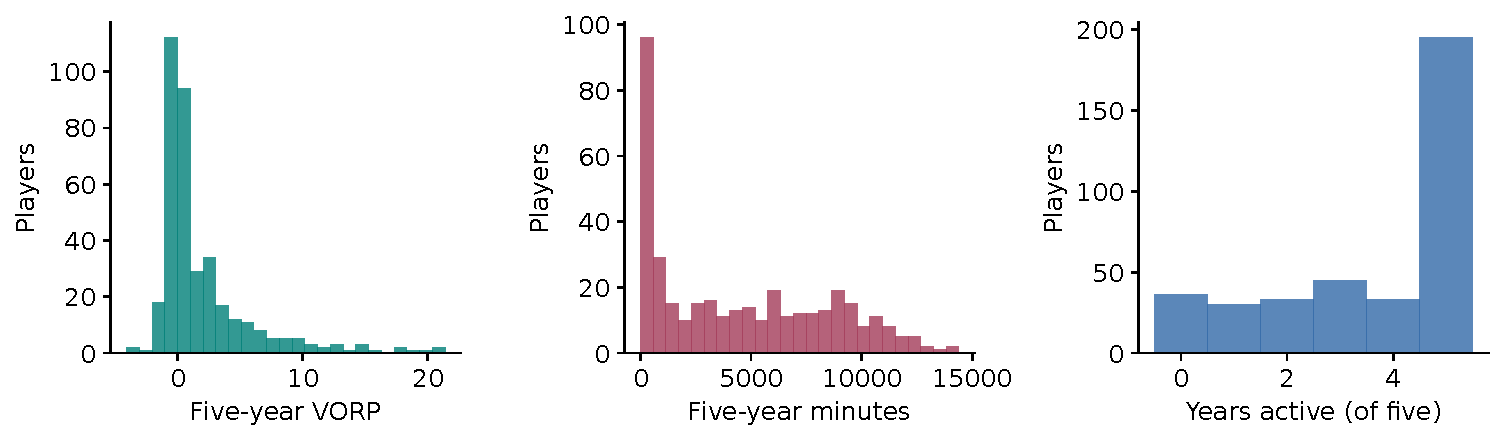
\includegraphics[width=\linewidth]{figures/outcome_distributions.pdf}
\caption{Development-pool outcomes with completed five-season follow-up by the 2020 origin. These are five-year cumulative value, opportunity, and restricted durability, not comparable units of one latent quantity.}
\end{figure}

College BPM and professional VORP can be examined together without assuming a deterministic translation. Exposure, role, program environment, and early recognition all confound a causal reading. Similarly, class-year distributions describe players already selected by NBA teams; a freshman--senior difference cannot show that staying in college causes a career outcome.

\begin{figure}[htbp]
\centering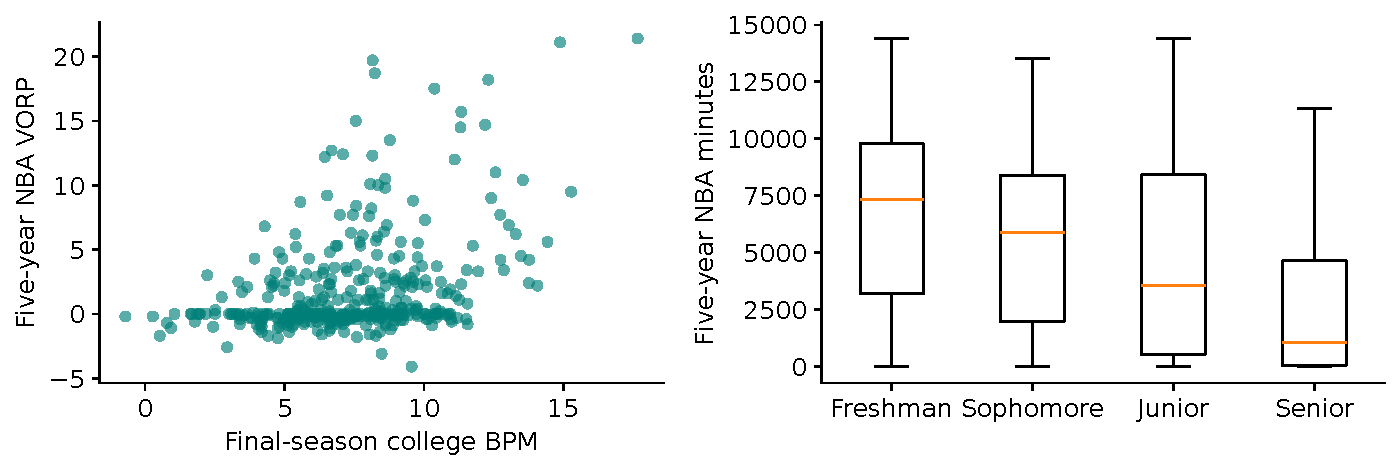
\includegraphics[width=.96\linewidth]{figures/college_relationships.pdf}
\caption{Descriptive development relationships: college BPM versus professional VORP, and five-year minutes by final college class. Box plots omit displayed outliers only; no player is removed from modeling.}
\end{figure}

Combine missingness is substantial for some drills and can reflect reporting conventions or participation choices. The model receives training-fold missingness indicators rather than zero-filled measurements. In contrast, actual zero shooting attempts and defensive events remain genuine zeros. These distinctions are important when evaluating whether a physical-feature gain reflects tools or participation patterns.

\begin{figure}[htbp]
\centering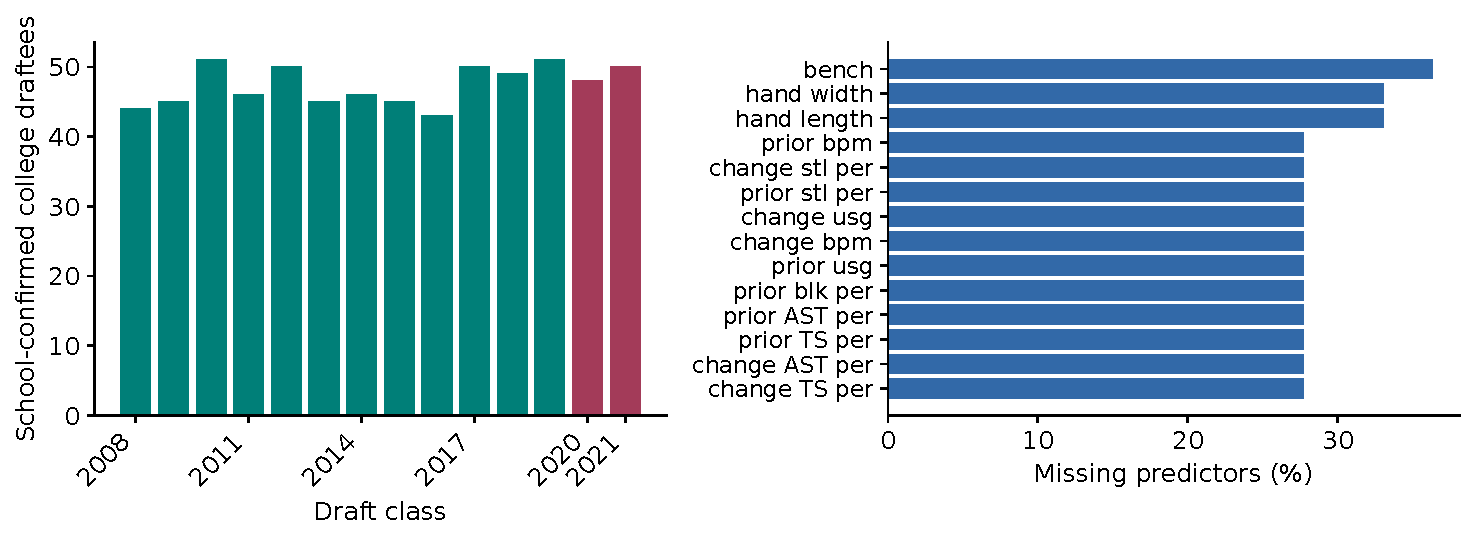
\includegraphics[width=\linewidth]{figures/cohort_missingness.pdf}
\caption{Left: eligible cohorts, with the final test in a distinct color. Right: the most frequently missing predictors in the mature development pool. Missingness is not used to discard otherwise eligible players.}
\end{figure}

\section{Methodology}
\subsection{Feature Sets}
The \emph{college} set contains 27 numeric predictors plus conference: height, games, playing time, minutes share, offensive rating, usage, efficiency, shooting percentages, rebounding, assists, turnovers, steals, blocks, free-throw rate, college BPM components, per-game production, and class year. Class year is a developmental proxy, not an exact age. Birth dates are not fabricated from later professional biographies.

The \emph{engineered} set adds six per-40 production measures, shot attempts per 40 minutes, attempt-weighted shooting stabilization, three-point attempt share, assist-to-turnover rate, defensive stocks, a usage--efficiency interaction, log exposure, prior college history, last-minus-prior changes, and teammate BPM. For shooting type $k$, stabilization uses
\begin{equation}
\widetilde p_{ik}=\frac{m_{ik}+\lambda_k p_{0k}}{a_{ik}+\lambda_k},
\end{equation}
where $m$ and $a$ are made and attempted shots. Fixed priors are $(p_0,\lambda)=(0.35,50)$ for threes, $(0.70,30)$ for free throws, and $(0.50,50)$ for twos. These conservative constants are not estimated using held-out outcomes. Missing inputs remain missing; zero attempts appropriately return the prior.

Prior performance summaries use only earlier seasons for the same college identifier and are weighted by games times minutes per game. Trajectories include BPM, usage, true shooting, assists, steals, and blocks. The panel begins in 2008: all 44 draftees in that class have no observed earlier season, including 33 nonfreshmen. A zero history count can therefore indicate left truncation rather than a first college season. Teammate context uses the same season's college roster, weighted by exposure and excluding the prospect; missing roster BPM contributes zero to its weighted numerator while exposure remains in the denominator, an additional approximation. The whole amateur roster concerns pre-draft seasons; professional outcomes never enter its calculation.

The \emph{hybrid} set adds 12 exact-draft-year combine measurements, position, wingspan surplus, BMI, jump gain, and maximum touch height. Implausible physical values become missing under broad fixed bounds. Eventual draft pick, an undocumented embedded recruiting rank, names, professional identifiers, cohort year, and all professional statistics are excluded from primary predictors. International production, injury histories, and contemporaneous scouting consensus lack sufficiently complete verified sources and are not imputed from future careers.

\subsection{Models and Hyperparameter Search}
We compare a training mean or prevalence constant; Ridge and Elastic Net regression or regularized logistic classification; Random Forest; Extra Trees; XGBoost; LightGBM; and CatBoost. Numeric predictors undergo median imputation, explicit missingness indicators, and standardization. Conference and position use training-fitted one-hot encodings with unknown categories tolerated. Every fitted operation occurs within the relevant training fold; there is no global VIF pruning, full-sample scaling, or outcome-informed feature screen.

Each nonconstant family receives 12 configurations generated with random seed 199, spanning feature set and regularization or tree complexity. Forests use 200 trees, depth 3, 5, 8 or unrestricted, minimum leaf size 3, 5, 10 or 15, and feature fraction 0.4, 0.7 or 1.0. Boosters explore shallow trees, conservative learning rates, iteration counts, and regularization. Regression compares raw targets, fixed asinh transforms, and training-fitted Yeo--Johnson transforms; validation always scores inverse-transformed predictions on the original target scale. The asinh inverse clips transformed predictions to $[-12,12]$ before applying $\sinh$ as a numerical guard. Nonlinear inversion does not generally recover the original-scale conditional mean, so transformed-scale fit alone is not evidence of better squared-error prediction. Convergence failures or nonfinite predictions disqualify candidates and remain in the log.

A three-family ensemble averages predictions from the three best nonconstant families within each inner tuning procedure. The weights are equal, not fitted to the final test. The constant remains eligible for primary selection. We also freeze the best development-selected candidate within each feature group for ablation. A separate one-variable draft-order Ridge or logistic model provides a meaningful professional-consensus benchmark; its actual draft number is unavailable before selection, so it is not an admissible primary predictor.

\subsection{Maturity-Gap Chronological Validation}
At prediction year $t$, a training record is eligible only when its five-season observation window is complete, $d_i+5\leq t$. An inner validation year $v$ is eligible for tuning only if $v+5\leq t$, and its fitting classes satisfy $d_i+5\leq v$. Thus even chronological adjacent-class validation would use future long-horizon outcomes if it omitted the maturity gap. The rule constrains follow-up completion; historical availability of the metric definitions and archived source releases is a separate, incompletely verified condition.

Nested outer diagnostics forecast the 2018 and 2019 draft classes. The 2018 procedure tunes on class 2013, trained through 2008; the 2019 procedure tunes on classes 2013--2014, each with its own gap. The outer fitting pools extend through 2013 and 2014, respectively. Those outer outcomes mature in 2023--2024 and cannot select a final model at the 2020 origin. Moreover, an earlier reconstruction in this project had already evaluated 2018--2019 under a different combine-based population and outcome definition. These classes therefore provide retrospective procedure diagnostics, not a fresh independent confirmation of the revised research design.

The final 2020 family and hyperparameter selection uses classes 2013--2015 as inner validation, trained through 2008--2010, respectively. All those validation labels mature by 2020. Its frozen specifications are fit through class 2015 to forecast 2020, then refit unchanged through class 2016 to forecast 2021. The 2020 and 2021 outcomes cannot enter either training pool. The five-year delay produces small early fitting pools even though the full reconstructed dataset is larger; this is a genuine limitation of historical long-term forecasting.

\begin{table}[htbp]
\centering\small
\begin{tabular}{llll}
\toprule
Forecast origin & Inner validation & Inner fit ends & Outer / final fit ends\\
\midrule
2018 & 2013 & 2008 & 2013\\
2019 & 2013, 2014 & 2008, 2009 & 2014\\
2020 & 2013, 2014, 2015 & 2008, 2009, 2010 & 2015\\
2021 & Specifications frozen in 2020 & No new tuning & 2016\\
\bottomrule
\end{tabular}
\caption{The information clock. A validation outcome must be mature at the selection origin, and a fitting outcome must be mature at its own forecast origin.}
\end{table}

\subsection{Selection, Scoring, and Uncertainty}
Regression selects the smallest pooled mean squared error, reporting original-scale RMSE, MAE, $R^2$, and Spearman correlation. Years active is modeled as a continuous response despite its integer range of zero to five. Frozen regression outputs are unconstrained and are scored without clipping: the selected nested procedure produces one value above five, and some supplementary models produce negative minutes or active-year predictions above five. These outputs are numerical forecasts, not admissible realized counts. A bounded procedure would require a separately declared analysis and independent evaluation. Classification selects the smallest pooled Brier score,
\begin{equation}
\operatorname{BS}=\frac{1}{n}\sum_i(y_i-\widehat p_i)^2,
\end{equation}
with log loss, ROC AUC, average precision, prevalence, and calibration diagnostics also exported. No test-optimized probability threshold is used. Ranking targets by development skill $1-L_{\rm selected}/L_{\rm constant}$ describes predictability relative to a corresponding constant; it does not make different outcomes equally useful or create a common uncertainty scale.

The final evaluation is write-once. Before the recorded scoring run, source snapshots, processed inputs, configuration, research code, frozen specifications, and fitted models receive cryptographic hashes. The freeze was created on October 9, 2026, at 21:33:17 UTC; the recorded evaluation followed at 21:33:49 UTC. These are actual execution dates, whereas 2020 and 2021 are simulated forecast origins. The receipt binds the freeze, predictions, summaries, and score table. Reruns retain this evidence, and report generation checks it before creating publication assets. Documented amendments are confined to publication and integrity checks; fitting and selection remain unchanged. This local freeze establishes reproducibility of the recorded run, not public preregistration or proof that historical outcomes were never seen during project development. All-family and feature-ablation test tables are descriptive comparisons, not another opportunity for model selection.

We bootstrap 2,000 paired replicates by first resampling the two draft classes and then players within each selected class. Each replicate compares selected and baseline predictions on identical rows. Error and baseline-minus-selected intervals are conditional on these classes and fixed fitted models. Two cohorts cannot characterize broad future-era drift, refitting variation, or full uncertainty after model and target search. We make no confirmatory significance claim from these intervals.

\section{Results}
\subsection{Development Selection}
The completed search logs \TrialN{} candidate evaluations across five targets and three tuning origins. Each entry records its features, transformation, parameters, validation loss, and any failure. The most favorable development-relative skill belongs to \FocalTarget{}, but every target in the recorded frozen implementation is retained. The scores below select final specifications using only the 2013--2015 labels mature at the 2020 origin; they are not unbiased final-performance estimates.

\begin{table}[htbp]
\centering\small\begin{tabular}{lrl}
\toprule
Target & Development skill & Frozen selection \\
\midrule
Five-year VORP & 0.150 & Regularized linear \\
Five-year minutes & 0.215 & Three-family ensemble \\
Years active (of five) & 0.174 & Three-family ensemble \\
Sustained rotation & 0.087 & Three-family ensemble \\
Sustained starter & 0.086 & Extra Trees \\
\bottomrule
\end{tabular}
\caption{Final development selection. Skill is relative reduction in MSE or Brier score against the constant on the same mature inner cohorts; the five outcomes have different units and utilities.}
\end{table}

\begin{figure}[htbp]
\centering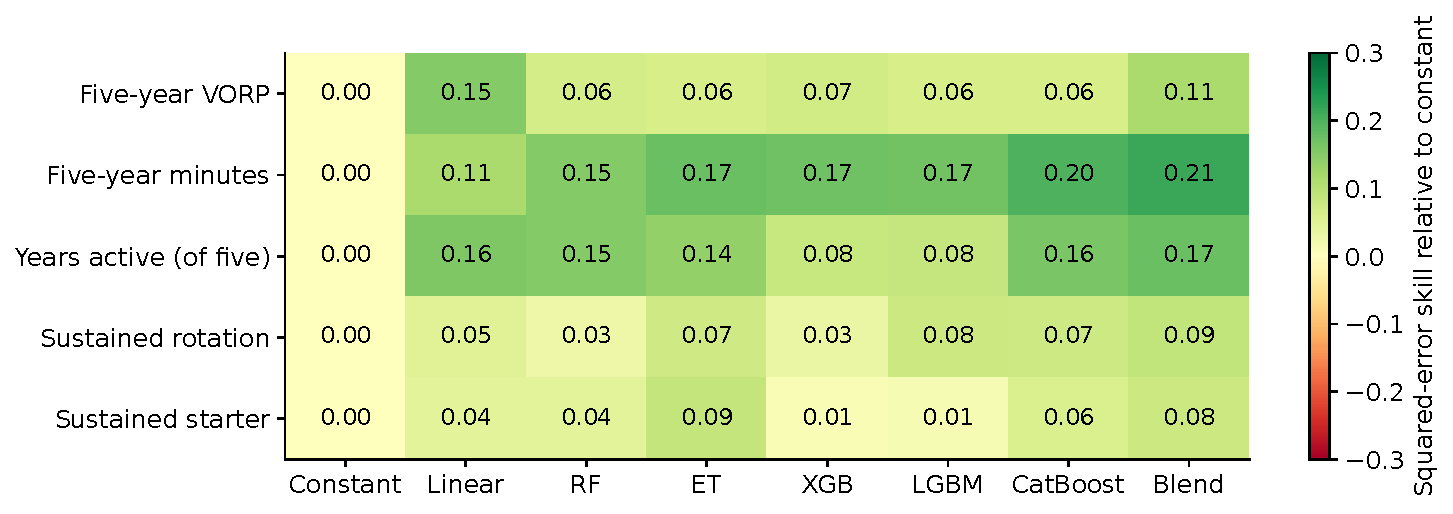
\includegraphics[width=\linewidth]{figures/development_comparison.pdf}
\caption{Best configuration per family on final development folds. Positive skill indicates improvement over the training mean or prevalence, not independent confirmation. The ensemble uses three nonconstant family finalists.}
\end{figure}

\subsection{Nested Procedure Diagnostics}
The nested forecasts of the 2018--2019 cohorts are shown separately. Each outer forecast includes family and configuration selection conducted using only labels with completed follow-up at its origin. These later labels do not determine the final 2020 specification. Differences between nested and development rankings reveal the instability of a small historical selection problem, rather than providing a reason to retune on future outcomes.

\begin{table}[htbp]
\centering\small\begin{tabular}{lrrrr}
\toprule
Target & $N$ & Selected error & Constant error & $R^2$ / AUC \\
\midrule
Five-year VORP & 100 & 3.086 & 3.250 & 0.089 \\
Five-year minutes & 100 & 3,086 & 3,418 & 0.186 \\
Years active (of five) & 100 & 1.297 & 1.433 & 0.054 \\
Sustained rotation & 100 & 0.210 & 0.245 & 0.724 \\
Sustained starter & 100 & 0.214 & 0.210 & 0.639 \\
\bottomrule
\end{tabular}
\caption{Pooled nested outer diagnostics. Error is RMSE for continuous outcomes and Brier score for binary outcomes. Final family selection does not use this table.}
\end{table}

\subsection{Frozen 2020--2021 Evaluation}
The final test contains \TestN{} school-confirmed NCAA draftees, 48 from 2020 and 50 from 2021. The selected models were frozen before these outcomes were scored. Table~\ref{tab:holdout} compares the selected procedure against a correspondingly refit constant. Supplementary comparisons include all frozen family finalists, feature-group ablations, and actual draft order; none is promoted based on its final-test performance.

\begin{table}[htbp]
\centering\footnotesize\begin{tabular}{llrrr}
\toprule
Target & Frozen selection & Error & Constant & $R^2$ / AUC \\
\midrule
Five-year VORP & Regularized linear & 3.664 & 3.655 & -0.007 \\
Five-year minutes & Three-family ensemble & 3,444 & 3,531 & 0.046 \\
Years active (of five) & Three-family ensemble & 1.459 & 1.509 & 0.015 \\
Sustained rotation & Three-family ensemble & 0.227 & 0.240 & 0.631 \\
Sustained starter & Extra Trees & 0.176 & 0.172 & 0.646 \\
\bottomrule
\end{tabular}
\caption{Frozen final-test performance. Error is original-scale RMSE for VORP, minutes, and years active, and Brier score for rotation and starter status. The last column is $R^2$ for regression and ROC AUC for classification.}
\label{tab:holdout}
\end{table}

The development-selected VORP specification is a college-only Ridge model with a training-fitted Yeo--Johnson target and penalty $\alpha=26.0823$. Its final-test RMSE is 3.664, slightly higher than the training-mean RMSE of 3.655, with $R^2=-0.007$. MAE decreases from 2.604 to 2.174, and Spearman correlation is 0.270. Lower absolute error and some ranking signal coexist with failure to improve the primary squared-error objective. This result does not demonstrate better prediction of high-value prospects.

The selected minutes ensemble yields RMSE 3,444 versus 3,531 for the constant, with $R^2=0.046$. The years-active ensemble yields RMSE 1.459 versus 1.509 and $R^2=0.015$. The rotation ensemble improves the Brier point estimate from 0.240 to 0.227, with AUC 0.631 and average precision 0.566 against prevalence 0.398. The hybrid Extra Trees starter model yields Brier 0.176 versus 0.172 for the constant, despite AUC 0.646. Discrimination alone does not establish improved probability accuracy.

All five paired constant-minus-selected bootstrap intervals include zero. These results support small and uncertain service-outcome point-estimate gains, not robust superiority across future draft classes. Nested outer comparisons improve on constants for VORP, minutes, active years, and rotation, but not for starter Brier score. Their different relationship to the final test reinforces the limits of transferring early-cohort selection.

Actual draft order is a substantially stronger benchmark for service outcomes on this test: rotation AUC is 0.821 with Brier 0.168, starter AUC is 0.817 with Brier 0.132, and minutes RMSE is 2,793 with $R^2=0.373$. VORP draft-order RMSE is 3.396 with $R^2=0.134$. This does not license adding eventual pick number to a pre-selection model; it instead shows that public college production and physical measurements do not replace the information and allocation processes summarized by the draft.

Feature ablations do not show a universal gain from complexity. Hybrid VORP RMSE is 3.636 versus 3.664 for the college-only ablation, while hybrid minutes RMSE is 3,643 versus 3,395 for college-only. Those supplementary scores are not used to substitute a new test-selected model. Development choice, not final-test ranking, determines every reported primary forecast.


\begin{figure}[htbp]
\centering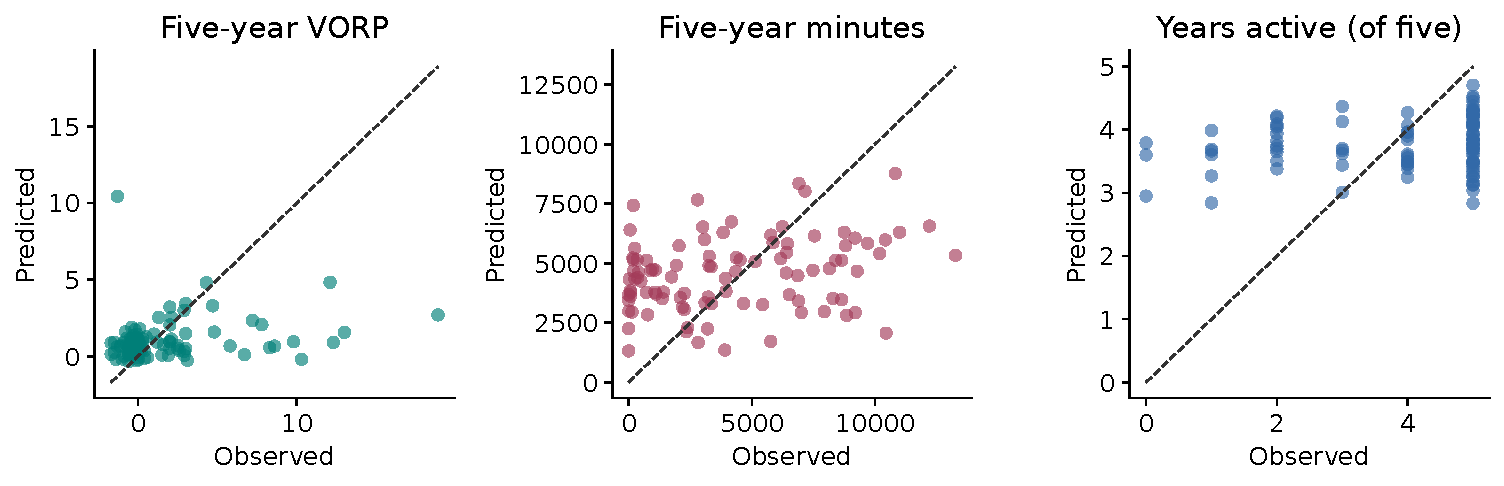
\includegraphics[width=\linewidth]{figures/test_regression.pdf}
\caption{Frozen regression predictions against observed five-year outcomes. The dashed line is identity, not a fitted calibration correction. High-value misses affect squared error substantially.}
\end{figure}

\begin{figure}[htbp]
\centering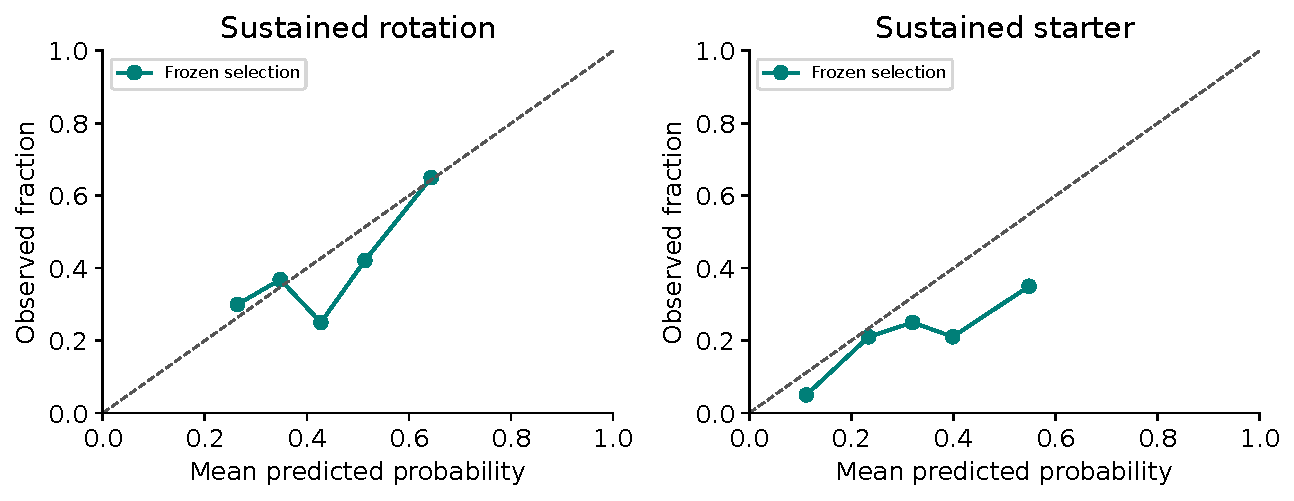
\includegraphics[width=.94\linewidth]{figures/test_calibration.pdf}
\caption{Binary calibration in five quantile bins on the final test. Small bins and two cohorts limit precision; these curves do not fit or recalibrate the model. AUC measures discrimination, not probability calibration.}
\end{figure}

\begin{table}[htbp]
\centering\small\begin{tabular}{lrr}
\toprule
Target & Error interval & Constant minus selected \\
\midrule
Five-year VORP & [2.523, 4.994] & [-0.688, 0.574] \\
Five-year minutes & [2,806, 4,084] & [-334, 531] \\
Years active (of five) & [1.287, 1.628] & [-0.021, 0.132] \\
Sustained rotation & [0.197, 0.262] & [-0.016, 0.039] \\
Sustained starter & [0.125, 0.241] & [-0.039, 0.029] \\
\bottomrule
\end{tabular}
\caption{Conditional 95\% hierarchical-bootstrap intervals. A positive constant-minus-selected interval favors the selected model. Units follow each target's RMSE or Brier score. These are not simultaneous intervals across targets.}
\end{table}

\begin{figure}[htbp]
\centering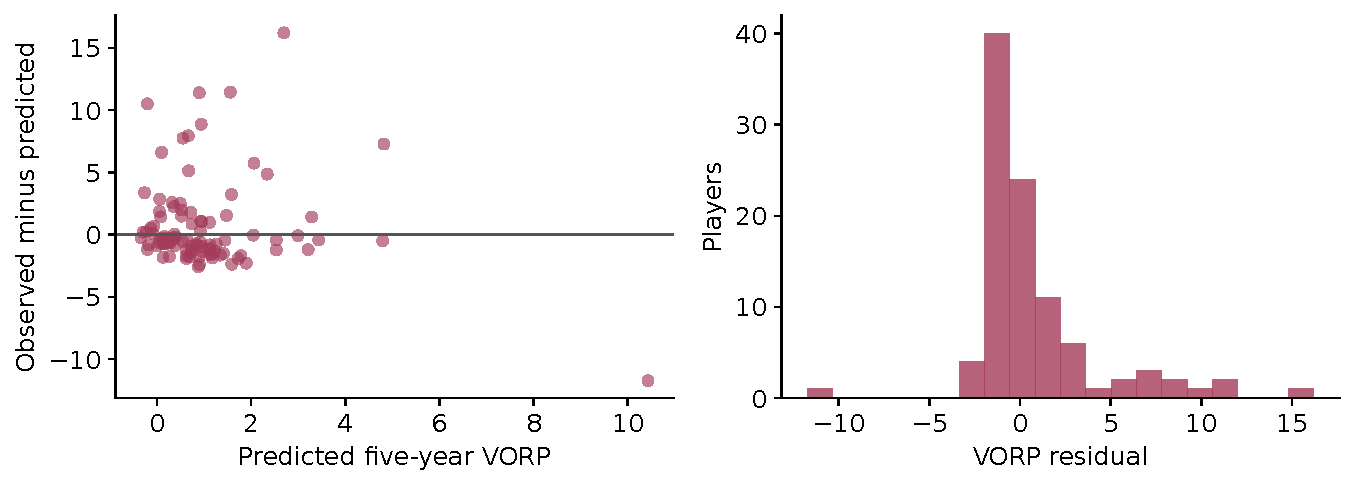
\includegraphics[width=.96\linewidth]{figures/residuals.pdf}
\caption{Final-test VORP residual diagnostics. These are held-out errors, not training residuals. They do not justify changing the fitted model after test evaluation.}
\end{figure}

\subsection{Interpretability Diagnostics}
The interpretability diagnostic uses the 2020-fitted Random Forest finalist with engineered predictors and an asinh target, fit on draft classes through 2015. Contributions are measured on the asinh-transformed scale. The primary VORP selection is Ridge; this forest is a separate retrospective diagnostic.
The diagnostic cohort is 2019 and contains different players from the fitting pool. This is a retrospective explanation of the 2020-fitted forest, not a forecast made at the 2019 origin: the class-2015 fitting outcomes complete their five-season window in 2020. Neither this analysis nor the permutation diagnostic supplies an independent chronological validation of the selected procedure. TreeSHAP contributions describe how this specific forest distributes a prediction across encoded predictors. Missingness indicators and one-hot conference levels remain visible rather than being disguised as biological traits. Contributions from correlated college metrics can substitute for each other; they do not isolate independent causal effects.

\begin{figure}[htbp]
\centering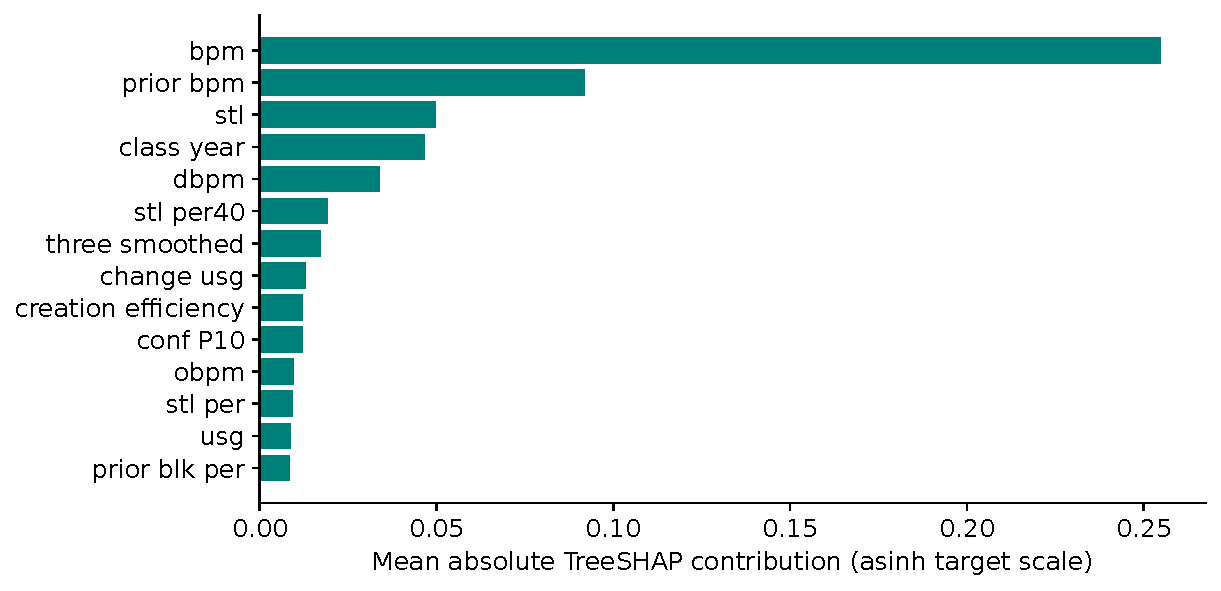
\includegraphics[width=.87\linewidth]{figures/shap_diagnostic.pdf}
\caption{Mean absolute TreeSHAP contributions for the VORP Random Forest finalist, fit for 2020 and explained retrospectively on the 2019 cohort. Target-scale units are printed on the axis. This is an explanation of a fitted finalist, not proof of a general trait hierarchy.}
\end{figure}

Permutation importance evaluates increases in original-scale VORP MSE on the same retrospective diagnostic cohort. Correlated predictors can dilute importance, and permutation can produce unrealistic combinations. The standard deviation of repeated permutations measures perturbation variability, not a population confidence interval. Negative values indicate that a feature's use does not reliably help on this cohort.

\begin{figure}[htbp]
\centering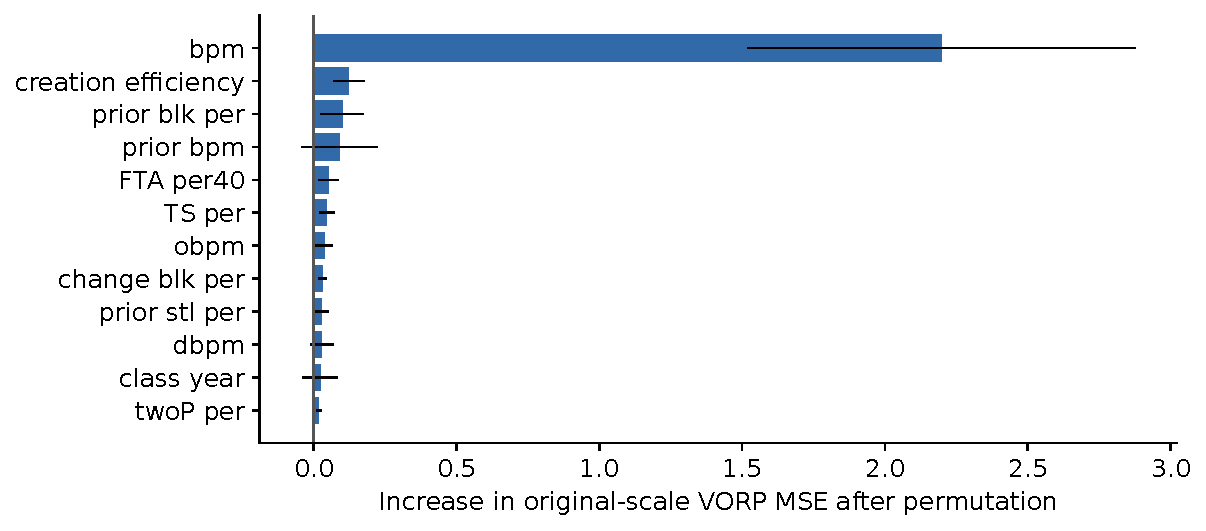
\includegraphics[width=.87\linewidth]{figures/permutation_diagnostic.pdf}
\caption{Retrospective diagnostic permutation importance for the 2020-fitted forest finalist on the 2019 cohort, measured on the original VORP scale. Bars show mean MSE increases; error bars show the standard deviation across 20 permutations.}
\end{figure}

\section{Discussion}
The study separates three questions that are often collapsed: whether public amateur data contains signal, whether a particular tuned procedure exploits that signal out of sample, and whether the procedure improves a real draft decision. A model can beat a constant without outperforming draft consensus, and a model can forecast minutes without identifying efficient or high-impact players. The final empirical comparisons support only the claims stated with the actual results above.

The feature comparisons offer no consistent case for adding complexity. Each feature-group finalist was tuned separately, so these are comparisons of modeling procedures, not controlled estimates of a single feature's marginal contribution. With small validation cohorts, differences can reflect specification choice and sampling variation as well as additional information. Combine missingness may encode participation or reporting patterns; it cannot be interpreted as a physiological mechanism.

The final selection uses only three mature inner cohorts, with early fitting pools of 44, 89, and 140 players. This is much less information than a random split of the full \SampleN{}-player archive would appear to offer. That limitation is not resolved by more trees, hundreds of optimizer trials, or assigning older players' current-career labels to an earlier prediction date. A stronger archive extending much further backward would improve the reliability of long-horizon selection.

The draft-order benchmark is valuable because it summarizes scouting and professional decisions omitted from public college statistics. It also embeds allocation effects: earlier picks may receive more opportunity. Its performance cannot distinguish teams identifying talent from teams creating opportunity. Since actual pick number is unavailable to a pre-selection decision, a model using it is a different tool, suitable for post-selection forecasting rather than independent draft ranking.

The negative VORP result does not contradict earlier evidence that college statistics are associated with NBA outcomes. Association, prediction after NBA entry, and improvement over a historical training mean under a strict information clock are different claims. Likewise, these small samples do not show that forests or boosting are generally inferior to linear models. The experiment evaluates a finite search over public predictors, not all usable scouting information.

Practical use should preserve the separate outputs. Estimated VORP describes realized box-score value; minutes and service probabilities describe participation and opportunity. Turning them into a draft board would require an explicit decision objective and prospective validation. The current results do not support using the models as a validated decision system.

\section{Limitations}
\textbf{Population and linkage.} The analysis is limited to drafted players with a recent, confirmed NCAA season. It does not represent all college players, undrafted entrants, high-school-only prospects, or international development pathways. Name-and-school joins materially strengthen college identity, but do not constitute birth-date-level linkage for every athlete. A post-evaluation audit identifies 12 candidate same-school naming variants among excluded records. Independent primary biographies corroborate these aliases, and 11 also agree with the archive's eventual draft-pick field. The latter is retrospective corroboration, not an admissible primary feature; this convenience investigation is not exhaustive adjudication of all exclusions. The frozen population remains 663 players, and excluded candidates are preserved for a future corrected reconstruction. Two common-name cases and two preexisting professional conflicts are excluded. Forty-one absent NBA records receive assumed zeros; unrecognized aliases remain a possible source of outcome error.

\textbf{Source verification.} Dated season fields prevent using later college seasons, but archived retrospective snapshots are not historical point-in-time database releases. Agreement between mirrored copies is not independent verification, and the independent ESPN checks are a small convenience sample. VORP is not independently reconstructed or audited against a second original provider. Basketball Reference introduced its original BPM in 2014 and BPM version 2.0 in February 2020; VORP derives from BPM \cite{bref}. The archived values' exact metric vintage has not been independently established. Completed five-season follow-up therefore does not demonstrate that the same VORP definition was available at the earlier simulated origins. College advanced-metric vintages and combine collection time are also incompletely documented, and archived fields can be revised. These limitations prevent a claim of a completely verified historical information set.

\textbf{Target scope.} Five-year longevity is not full career duration. Minutes, starts, and VORP depend on opportunity, injuries, contracts, coaches, teammates, and team quality. Fixed thresholds can penalize shortened seasons. Defensive value not captured by box scores, postseason contribution, development after year five, and salary-adjusted surplus are outside the estimand.

\textbf{Selection and uncertainty.} Family, transformation, feature, and target comparisons increase selection risk. Search is finite rather than exhaustive, nested outer diagnostics cover only two cohorts, and final tuning relies on three much earlier validation classes. The final test is held out under this protocol but historical, not a registered prospective trial. Conditional bootstrap intervals do not capture future regime changes, model-refitting variation, or simultaneous uncertainty after all comparisons. No claim of universal optimality follows from a finite model search.

\textbf{Transport and omitted predictors.} Pandemic-era cohorts, changes in three-point emphasis, transfer rules, college compensation, and alternative development routes can change translation to the NBA. Verified ages, recruiting trajectories, injury history, international production, and dated scouting consensus would be useful additions, but are not manufactured here. Acquiring them requires a new development cycle and independent future test, not repeated use of the consumed 2020--2021 outcomes.

\section{Conclusion}
We reconstruct dated college records and forecast five five-year NBA outcomes for drafted NCAA players. Requiring mature labels at every fitting and selection date sharply reduces the usable historical sample. The resulting baseline comparisons reveal how limited the gains from this public-data procedure are under that constraint.

The frozen evidence does not establish a reliable VORP accuracy improvement over a training mean. Small point-estimate improvements for minutes, restricted longevity, and rotation service remain uncertain; the starter probability model does not beat its constant on Brier score. Actual draft order remains substantially more informative for service outcomes, although it belongs to a later information set. These findings favor cautious, target-specific research use rather than a claim that a complex public-data model has solved draft evaluation.


Earlier independently verified amateur records, dated scouting information, and future cohorts would permit a stronger study. Any revised predictor or selection procedure must be evaluated on new data; the consumed 2020--2021 test cannot supply that evidence.

\section*{Reproducibility and Data Availability}
The local bundle contains code, snapshots, processed data, trial logs, frozen models, predictions, publication assets, and pinned dependencies. Large inputs and outputs are excluded from Git; a clone alone cannot reproduce the results, and no public persistent bundle identifier is available. Reruns preserve the consumed evaluation. Independent refits reproduce selected predictions; a separate audit reconstructs all targets and recalculates metrics and intervals from recorded snapshots. These checks establish numerical consistency, not provider accuracy. A separately dated October 13, 2026 audit seal binds 203 recorded inputs and evidence files, including development logs and split records; it is retrospective and does not amend the original freeze or establish preregistration. The added source and linkage checks are explicitly post-evaluation. Every manuscript page is rendered for layout review. Provider permissions and a persistent archival deposit remain necessary before public redistribution of third-party snapshots.

\clearpage
\appendix
\section{Frozen Specifications}
{\raggedright
\paragraph{Five-year VORP} Regularized linear; college predictors; yeojohnson target.\par {\small\raggedright \texttt{alpha}: 26.0823; \texttt{kind}: ridge.\par}
\paragraph{Five-year minutes} Equal-weight blend of three separately fitted finalists, averaged on the original outcome scale.
\begin{itemize}\small\raggedright
\item CatBoost; engineered predictors; raw target.\par \texttt{depth}: 4; \texttt{iterations}: 150; \texttt{l2\_leaf\_reg}: 50; \texttt{learning\_rate}: 0.1.
\item Extra Trees; engineered predictors; raw target.\par \texttt{max\_depth}: None; \texttt{max\_features}: 1; \texttt{min\_samples\_leaf}: 10; \texttt{n\_estimators}: 200.
\item XGBoost; hybrid predictors; raw target.\par \texttt{colsample\_bytree}: 0.8; \texttt{learning\_rate}: 0.1; \texttt{max\_depth}: 3; \texttt{min\_child\_weight}: 5; \texttt{n\_estimators}: 350; \texttt{reg\_lambda}: 20; \texttt{subsample}: 0.85.
\end{itemize}
\paragraph{Years active (of five)} Equal-weight blend of three separately fitted finalists, averaged on the original outcome scale.
\begin{itemize}\small\raggedright
\item CatBoost; college predictors; raw target.\par \texttt{depth}: 4; \texttt{iterations}: 150; \texttt{l2\_leaf\_reg}: 20; \texttt{learning\_rate}: 0.05.
\item Regularized linear; engineered predictors; yeojohnson target.\par \texttt{alpha}: 0.801525; \texttt{kind}: elastic; \texttt{l1\_ratio}: 0.1.
\item Random Forest; engineered predictors; raw target.\par \texttt{max\_depth}: None; \texttt{max\_features}: 0.7; \texttt{min\_samples\_leaf}: 5; \texttt{n\_estimators}: 200.
\end{itemize}
\paragraph{Sustained rotation} Equal-weight blend of three separately fitted finalists, averaged on the original outcome scale.
\begin{itemize}\small\raggedright
\item LightGBM; engineered predictors; raw target.\par \texttt{learning\_rate}: 0.02; \texttt{min\_child\_samples}: 10; \texttt{n\_estimators}: 350; \texttt{num\_leaves}: 3; \texttt{reg\_lambda}: 5.
\item CatBoost; engineered predictors; raw target.\par \texttt{depth}: 3; \texttt{iterations}: 150; \texttt{l2\_leaf\_reg}: 50; \texttt{learning\_rate}: 0.05.
\item Extra Trees; college predictors; raw target.\par \texttt{max\_depth}: 5; \texttt{max\_features}: 1; \texttt{min\_samples\_leaf}: 10; \texttt{n\_estimators}: 200.
\end{itemize}
\paragraph{Sustained starter} Extra Trees; hybrid predictors; raw target.\par {\small\raggedright \texttt{max\_depth}: None; \texttt{max\_features}: 0.7; \texttt{min\_samples\_leaf}: 10; \texttt{n\_estimators}: 200.\par}
}

\clearpage
\section{Supplementary Comparisons}
\begin{table}[htbp]
\centering\footnotesize\begin{tabular}{lrrrrr}
\toprule
Model & VORP & Minutes & Active & Rotation & Starter \\
\midrule
Training mean / prevalence & 3.655 & 3,531 & 1.509 & 0.240 & 0.172 \\
Regularized linear & 3.664 & 3,367 & 1.427 & 0.222 & 0.164 \\
Random Forest & 3.671 & 3,436 & 1.511 & 0.220 & 0.170 \\
Extra Trees & 3.667 & 3,437 & 1.480 & 0.231 & 0.176 \\
XGBoost & 3.636 & 3,643 & 1.464 & 0.219 & 0.172 \\
LightGBM & 3.668 & 3,453 & 1.560 & 0.227 & 0.169 \\
CatBoost & 3.640 & 3,415 & 1.492 & 0.232 & 0.167 \\
Three-family ensemble & 3.628 & 3,444 & 1.459 & 0.227 & 0.166 \\
draft order benchmark & 3.396 & 2,793 & 1.424 & 0.168 & 0.132 \\
ablation college & 3.664 & 3,395 & 1.492 & 0.231 & 0.180 \\
ablation engineered & 3.674 & 3,415 & 1.427 & 0.227 & 0.170 \\
ablation hybrid & 3.636 & 3,643 & 1.501 & 0.225 & 0.176 \\
\bottomrule
\end{tabular}
\caption{All frozen family finalists and feature-group ablations on the final test. Continuous columns are RMSE; binary columns are Brier scores. Draft order is a separately labeled post-selection benchmark. Models are displayed without test-score ranking or promotion.}
\end{table}

\begin{table}[htbp]
\centering\small\begin{tabular}{llrrr}
\toprule
Target & Draft & $N$ & Error & $R^2$ / AUC \\
\midrule
Five-year VORP & 2020 & 48 & 4.202 & -0.178 \\
Five-year VORP & 2021 & 50 & 3.060 & 0.200 \\
Five-year minutes & 2020 & 48 & 3,837 & -0.080 \\
Five-year minutes & 2021 & 50 & 3,018 & 0.193 \\
Years active (of five) & 2020 & 48 & 1.483 & 0.046 \\
Years active (of five) & 2021 & 50 & 1.435 & -0.030 \\
Sustained rotation & 2020 & 48 & 0.240 & 0.596 \\
Sustained rotation & 2021 & 50 & 0.215 & 0.641 \\
Sustained starter & 2020 & 48 & 0.213 & 0.580 \\
Sustained starter & 2021 & 50 & 0.140 & 0.765 \\
\bottomrule
\end{tabular}
\caption{Selected models by final-test draft class. Different class-level outcomes and errors illustrate why two classes do not establish future-era stability.}
\end{table}

\begin{table}[htbp]
\centering\footnotesize\setlength{\tabcolsep}{3pt}\begin{tabular}{llrrrrr}
\toprule
Target & Model & Prevalence & Brier & Log loss & AUC & AP \\
\midrule
Sustained rotation & selected & 0.398 & 0.227 & 0.645 & 0.631 & 0.566 \\
Sustained rotation & constant & 0.398 & 0.240 & 0.673 & 0.540 & 0.419 \\
Sustained rotation & draft order benchmark & 0.398 & 0.168 & 0.507 & 0.821 & 0.744 \\
Sustained starter & selected & 0.214 & 0.176 & 0.532 & 0.646 & 0.344 \\
Sustained starter & constant & 0.214 & 0.172 & 0.530 & 0.418 & 0.194 \\
Sustained starter & draft order benchmark & 0.214 & 0.132 & 0.407 & 0.817 & 0.602 \\
\bottomrule
\end{tabular}
\caption{Frozen binary probability and discrimination metrics. Lower Brier score and log loss are preferable; higher AUC and average precision (AP) are preferable. Prevalence supplies the no-skill reference for AP. Constants are refitted by forecast year, so pooled constant predictions need not be identical.}
\end{table}

\clearpage
\raggedright
\begin{thebibliography}{99}
\bibitem{coates} Coates, D., and Oguntimein, B. (2010). The length and success of NBA careers: Does college production predict professional outcomes? \emph{International Journal of Sport Finance}, 5(1), 4--26. Working-paper version: \url{https://college.holycross.edu/hcs/RePEc/spe/CoatesOguntimein_NBA.pdf}.
\bibitem{moxley} Moxley, J. H., and Towne, T. J. (2015). Predicting success in the National Basketball Association: Stability and potential. \emph{Psychology of Sport and Exercise}, 16, 128--136. \url{https://doi.org/10.1016/j.psychsport.2014.07.003}.
\bibitem{kannan} Kannan, A., Kolovich, B., Lawrence, B., and Rafiqi, S. (2018). Predicting National Basketball Association success: A machine learning approach. \emph{SMU Data Science Review}, 1(3), Article 7. \url{https://scholar.smu.edu/datasciencereview/vol1/iss3/7/}.
\bibitem{teramoto} Teramoto, M., Cross, C. L., Rieger, R. H., Maak, T. G., and Willick, S. E. (2018). Predictive validity of National Basketball Association draft combine on future performance. \emph{Journal of Strength and Conditioning Research}, 32(2), 396--408. \url{https://doi.org/10.1519/JSC.0000000000001798}.
\bibitem{li} Li, H., and Cao, Q. (2025). Evaluating the predictive power of NBA draft combine metrics on early-career performance: An empirical analysis from the 2022--2024 seasons. \emph{Advances in Economics, Management and Political Sciences}, 226, 83--96. \url{https://doi.org/10.54254/2754-1169/2025.LH27926}.
\bibitem{wiethuchter} Wieth\"uchter, C. F. (2025). \emph{Predicting Early NBA Career Survivability Using Pre-Draft College Statistics}. MSc dissertation, Universidade Cat\'olica Portuguesa. \url{https://hdl.handle.net/10400.14/55936}.
\bibitem{czasonis} Czasonis, M., Kritzman, M., Kulasekaran, C., and Turkington, D. (2024). \emph{How to Predict the Performance of NBA Draft Prospects}. MIT Sloan Sports Analytics Conference research paper, version January 31, 2024. \url{https://www.sloansportsconference.com/research-papers/how-to-predict-the-performance-of-nba-draft-prospects}.
\bibitem{milosevic} Milo\v{s}evi\'{c}, P., Milo\v{s}evi\'{c}, D., Milenkovi\'{c}, I., Dragovi\'{c}, I., Raki\'{c}evi\'{c}, A., and Zukanovi\'{c}, M. (2026). From rookie to contract extension: Modeling NBA player career trajectories with machine learning. \emph{Journal of Sports Analytics}, advance online publication. \url{https://doi.org/10.1177/22150218261484000}.
\bibitem{breiman} Breiman, L. (2001). Random forests. \emph{Machine Learning}, 45, 5--32. \url{https://doi.org/10.1023/A:1010933404324}.
\bibitem{xgboost} Chen, T., and Guestrin, C. (2016). XGBoost: A scalable tree boosting system. \emph{Proceedings of KDD}, 785--794. \url{https://doi.org/10.1145/2939672.2939785}.
\bibitem{lightgbm} Ke, G., et al. (2017). LightGBM: A highly efficient gradient boosting decision tree. \emph{Advances in Neural Information Processing Systems}, 30. \url{https://proceedings.neurips.cc/paper/2017/hash/6449f44a102fde848669bdd9eb6b76fa-Abstract.html}.
\bibitem{catboost} Prokhorenkova, L., Gusev, G., Vorobev, A., Dorogush, A. V., and Gulin, A. (2018). CatBoost: Unbiased boosting with categorical features. \emph{Advances in Neural Information Processing Systems}, 31. \url{https://arxiv.org/abs/1706.09516}.
\bibitem{cawley} Cawley, G. C., and Talbot, N. L. C. (2010). On over-fitting in model selection and subsequent selection bias in performance evaluation. \emph{Journal of Machine Learning Research}, 11, 2079--2107. \url{https://jmlr.org/papers/v11/cawley10a.html}.
\bibitem{shap} Lundberg, S. M., and Lee, S.-I. (2017). A unified approach to interpreting model predictions. \emph{Advances in Neural Information Processing Systems}, 30. \url{https://proceedings.neurips.cc/paper/2017/hash/8a20a8621978632d76c43dfd28b67767-Abstract.html}.
\bibitem{torvik} Torvik, B. College basketball player statistics. \url{https://barttorvik.com/playerstat.php}. Dated historical seasons preserved in archived source snapshots.
\bibitem{gonzaga} Gonzaga, M. \emph{NBADraftModel}: Archived Torvik-origin raw college seasons and field mapping. Commit \texttt{099a9fc5776a25d72ceae5fb9a8cb09b67890c1c}. \url{https://github.com/mathgonzaga/NBADraftModel}.
\bibitem{archive} \emph{NBA Role Player Prediction Model} public repository: Secondary college and NBA source CSV archives. Commit \texttt{0524c1e21992bc3e55197a467ead6e6262c4c200}. \url{https://github.com/warrensuca/nba-role-player-prediction-model}. Only raw source files, not this repository's fitted models, population filters, or outcome labels, are used.
\bibitem{espn} ESPN. Historical NBA draft archives and player season statistics. \url{https://www.espn.com/nba/draft/history}. Public JSON snapshots preserve draft years and regular-season records; source URLs and retrieval timestamps accompany the research inputs.
\bibitem{bref} Basketball Reference. NBA regular-season advanced statistics and Box Plus/Minus methodology. \url{https://www.basketball-reference.com/about/bpm2.html}. Source-origin attribution; direct retrieval was unavailable.
\bibitem{nba} NBA. Draft combine statistics. \url{https://www.nba.com/stats/draft/combine}. Physical measurements are taken from the exact actual-draft-year cached record.
\end{thebibliography}
\end{document}
